\documentclass[conference]{IEEEtran}
\IEEEoverridecommandlockouts
% The preceding line is only needed to identify funding in the first footnote. If that is unneeded, please comment it out.
\usepackage{booktabs}
\usepackage{diagbox}
\usepackage{hyperref}
\usepackage{CJKutf8}
\usepackage{cite}
\usepackage{amsmath,amssymb,amsfonts}
\usepackage{algorithmic}
\usepackage{graphicx}
\usepackage{textcomp}
\usepackage{xcolor}
\usepackage{listings}
\usepackage{color}

\definecolor{dkgreen}{rgb}{0,0.6,0}
\definecolor{gray}{rgb}{0.5,0.5,0.5}
\definecolor{mauve}{rgb}{0.58,0,0.82}

\lstset{frame=tb,
  language=Python,
  aboveskip=3mm,
  belowskip=3mm,
  showstringspaces=false,
  columns=flexible,
  basicstyle={\small\ttfamily},
  numbers=none,
  numberstyle=\tiny\color{gray},
  keywordstyle=\color{blue},
  commentstyle=\color{dkgreen},
  stringstyle=\color{mauve},
  breaklines=true,
  breakatwhitespace=true,
  tabsize=3
}
\def\BibTeX{{\rm B\kern-.05em{\sc i\kern-.025em b}\kern-.08em
    T\kern-.1667em\lower.7ex\hbox{E}\kern-.125emX}}
\begin{document}
\begin{CJK*}{UTF8}{bsmi}

\title{還錢啦乾\\
{\footnotesize \textsuperscript{*}Note: Sub-titles are not captured in Xplore and
should not be used}
\thanks{Identify applicable funding agency here. If none, delete this.}
}

\author{\IEEEauthorblockN{1\textsuperscript{st} 許呈孺}
    \IEEEauthorblockA{\textit{dept. Forestry} \\ 
    \textit{B11605076}}
\and
\IEEEauthorblockN{2\textsuperscript{nd} 王薏筎}
    \IEEEauthorblockA{\textit{dept. Forestry}\\
    \textit{B11605063}}
\and
\IEEEauthorblockN{3\textsuperscript{rd} 馬若恩}
    \IEEEauthorblockA{\textit{dept. Forestry}\\
    \textit{B11605005}}
\and
\IEEEauthorblockN{4\textsuperscript{th} 盧音佑}
    \IEEEauthorblockA{\textit{dept. Forestry}\\
    \textit{B11605085}}
\and
\IEEEauthorblockN{5\textsuperscript{th} 鄭捷安}
\IEEEauthorblockA{\textit{dept. Foresty} \\
    \textit{B10605090}}
\and
\IEEEauthorblockN{6\textsuperscript{th} 劉璟妮}
\IEEEauthorblockA{\textit{dept. Foresty} \\
    \textit{B09605042}}
}

\maketitle

\begin{abstract}
使用Python處理文字、紀錄多人間的債務關係。債務關係可以隨時更新、更改,並且有清算功能,分辨使用者分帳。
\end{abstract}

\begin{IEEEkeywords}
分帳,機器人,還錢,理財,欠錢
\end{IEEEkeywords}

\section{簡介}
每次跟朋友分帳都非常痛苦,目前大家都是打在Line群上用文字接龍來紀錄。

但這樣紀錄非常痛苦,雖然市面上有一些分帳程式,但沒有一個是功能很貼切我們需求的,所以希望能自己寫出一個客製化又介面化、人性化的程式幫我們算(畢竟能自己加功能才是真正客製化)。
\section{方法與素材}

\subsection{如何紀錄債務?}

假設有$N$個人,那麼就會有一個$N \times N$的字典,稱作$relation$,如此一來若要檢查欠債關係,直接用$relation[A][B]$來索引即可,若得到0就是沒有欠債關係,若是得到正數$m$就是[A]欠[B] m 塊錢,負數就是反向關係。

例如ABC三個人,A欠B一百塊,C欠A一百塊,關係如下:
\begin{lstlisting}
relation = {
        "A": {
            "A": 0,
            "B": 100,
            "C": -100,
            },
        "B": {
            "A": -100,
            "B": 0,
            "C": 0,
            },
        "C": {
            "A": 100,
            "B": 0,
            "C": 0,
            }
        }
\end{lstlisting}

\subsection{使用方式}

\begin{enumerate}
    \item 將文字輸入:\\ 
    如「阿靖欠良171」可以自動偵測「阿靖」欠「良」171塊(金額規定是數字)。\\ 
    並且預設是將原債務直接加上去,如A已經欠B一百塊,若再輸入A 欠 B 150,A就會總計欠B兩百五。

        詳細方式:
    \begin{enumerate}
    \item 單人欠單人:\\
    輸入:[$n_1$] 欠 [$m$] [amount],如此一來在程式中可以這樣做:

            \begin{lstlisting}
relation[n1][m] = [amount]
relation[m][n1] = -[amount]
            \end{lstlisting}

    即設置完債務關係。
    \item 多人欠單人:\\
        輸入:[$n_1$] [$n_2$] ...[$n_k]$ 欠 [$m$] [amount]

    這個情況預設為欠債人平分金額,一起欠債權人,在程式裡可以像這樣做:
            \begin{lstlisting}
split = amount / k 
for person in people:
    relation[person][m] = split
    relation[m][person] = -split
            \end{lstlisting}

    若是$m$其中有付自己的份,則輸入的金額要自己先減掉

    \item 多人欠多人:\\ 
        輸入:[$n_1$] [$n_2$] ... [$n_k$] 欠 [$m_1$] [$amount_1$] [$m_2$] [$amount_2$] …

    此情況不常出現,目前想法是直接將金額當作多欠單的方式平分下去,但要不要實作出來還在考慮
        
    \end{enumerate}    
  \item 直接在介面選擇欠債人跟債主,輸入金額\\ 
      主要使用介面見Fig. 1

        \begin{enumerate}
            \item 分為三大介面:欠錢、還錢、(功能區)。
            \item 人名選單設想為下拉是選單,且是誰欠錢可為複選(處理多欠一的情況)。
            \item 時間紀錄預設為記錄當下時區時間,並記錄在功能區中的歷史紀錄。
            
        \end{enumerate}

    \begin{figure}[htbp]
        \centerline{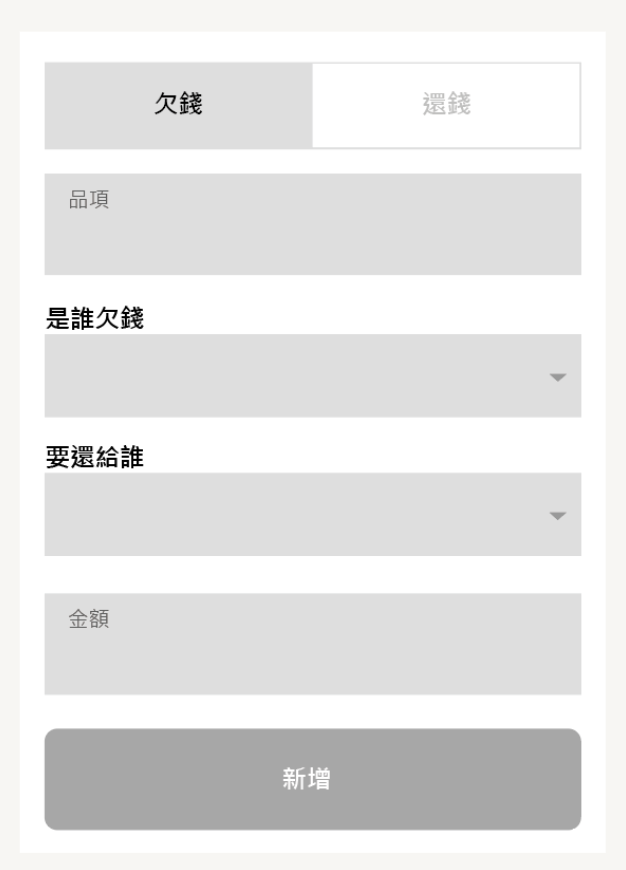
\includegraphics[height=0.5\textwidth]{gui.png}}
    \caption{理想中的介面}
    \label{fig}
    \end{figure}

\end{enumerate}


\section{預期功能}

列出所有債務功能,方便看出大家的債務關係(也方便debug)。

除了列出債務關係之外,因為我們的習慣是一個月結清一次債務,因此希望會有一個結清債務功能。

\subsection{列出債務}

簡單的用for loop列出每個人的債務即可:
\begin{lstlisting}
for person, debts in relation.items():
    print(f"{person}:")
    for m, debt in debts.items():
        print(f"\t{m}: {debt}")
\end{lstlisting}

\subsection{結清債務}\label{settle}
無論有多少筆帳,每個人最後的結餘只會有一個數字(實收多少或實付多少)。

綜觀來看,每個人都會有一個付出的金額,以及得到的金額價值,相減即是結輕的金額,金額是正的代表要付出金額,為負代表要收到金錢。

在程式中可以很簡單的用for loop來清算:

\begin{lstlisting}
for person, debts in relation.items():
    total = 0
    for debt in debts.values():
        total += debt
    print(f"{person}: {debt}")
\end{lstlisting}

\subsection{介面化}

介面化預計使用\href{https://docs.python.org/3/library/tkinter.html}{tkinter}。

但介面化的實用性實際上不大,因為這樣還是需要一個人操作電腦上的軟體。因此更實用的方法是做成Line Bot。

\subsection{Line Bot}

若將其實作成分帳Line Bot的話,就可以將它邀請進群組,並且直接在群組中輸入文字指令即可。

列出債務、清算功能也都是用文字輸出到群組。

在稍微瀏覽了一下\href{https://github.com/line/line-bot-sdk-python}{GitHub: line-bot-sdk-python}後目前認為此想法是可行,

\subsection{最少轉帳次數計算(考慮中)}

在使用結清功能後,雖然可以知道每個人的實收實付,但若不是所有人都在現場的話,就要使用轉帳來還錢,那麼我們可以用Minimum Cost Maximum Flow (MCMF) 找出最小轉帳次數及方式。

若結清後的輸出為:
\begin{lstlisting}
A: 500
B: -35
C: -215
D: -250
\end{lstlisting}
使用MCMF算出來的結果為:
\begin{lstlisting}
Minimum transaction: 3
B pay A 35
C pay A 215
D pay A 250
\end{lstlisting}
以上範例雖很簡單,但更複雜的情況MCMF就可以發揮其最大效用。

\section*{開發時程表}

\begin{table}[hbt!]
\begin{tabular}{|c|l|lll}
\cline{1-2}
    \\[-1em]
    Week & \multicolumn{1}{c|}{To-do}    &  &  &  \\ \cline{1-2}
    \\[-1em]
10   & 主程式開發:文字輸入處理、欠錢機制             &  &  &  \\ \cline{1-2}
\\[-1em]
11   & 功能開發:債務關係整理、清算功能、MCMF計算       &  &  &  \\ \cline{1-2}
\\[-1em]
12   & 延伸開發:Line Bot/介面化,連接後端\&前端    &  &  &  \\ \cline{1-2}
\\[-1em]
13   & 整理:Clean up code, refactoring &  &  &  \\ \cline{1-2}
\end{tabular}
\end{table}

\section*{分工表}

\begin{table}[hbt!]
\begin{tabular}{|c|c|lll}
\cline{1-2}
    \\[-1em]
組員                        & 工作                      &  &  &  \\ \cline{1-2}
    \\[-1em]
許呈孺                       & 監督、清算功能、MCMF算法、Line Bot &  &  &  \\ \cline{1-2}
    \\[-1em]
王薏茹                       & 介面、Line Bot             &  &  &  \\ \cline{1-2}
    \\[-1em]
馬若恩                       & 介面、Line Bot             &  &  &  \\ \cline{1-2}
    \\[-1em]
盧音佑                       & 文字輸入處理功能                &  &  &  \\ \cline{1-2}
    \\[-1em]
\multicolumn{1}{|l|}{鄭捷安} & 介面、文字輸入處理功能             &  &  &  \\ \cline{1-2}
    \\[-1em]
\multicolumn{1}{|l|}{劉璟妮} & 介面、文字輸入處理功能             &  &  &  \\ \cline{1-2}
\end{tabular}
\end{table}

\begin{thebibliography}{00}
\bibitem{b1} Lai, L. (2023, February 9). Lightsplit 最少轉帳次數研究實作. Larry’s Notes. https://www.larrysprognotes.com/Lightsplit/
\bibitem{b2} Wu, K. (2020, September 11). [實作]多人分帳程式 — 分帳邏輯及User Story. Medium.
\bibitem{b3} Wu, K. (2020, September 11). [實作]多人分帳程式(二) — JS陣列、物件概念. Medium.
\end{thebibliography}
\vspace{12pt}

\end{CJK*}
\end{document}
